\documentclass{article}
\usepackage{amsmath}
\usepackage{graphicx}
\usepackage{geometry}
\usepackage{xcolor} % for custom colors
\usepackage{float}       % for [H] placement
\usepackage{caption}     % for better caption control
\usepackage{subcaption} 
\usepackage{listings}

\lstset{
  language=Python,
  basicstyle=\ttfamily\small,
  keywordstyle=\color{blue}\bfseries,
  stringstyle=\color{red},
  commentstyle=\color{green!50!black},
  numbers=left,
  numberstyle=\tiny,
  stepnumber=1,
  numbersep=10pt,
  backgroundcolor=\color{gray!10},
  frame=single,
  breaklines=true,
  captionpos=b,
  tabsize=4,
  showspaces=false,
  showstringspaces=false
}

\geometry{a4paper, margin=1in}

\title{Homework 2}
\author{Your Name}
\date{\today}

\begin{document}

\maketitle


We will now start reflecting on the coding questions of Homework 2. The code base that can be used to replicate the result can be found
in the following link: \texttt{https://github.com/TagoreZhao/STAT260/tree/main/HW2}

\section{Problem 6, 7, and 8}

The code needed for generating these three matrices is given below:

\begin{lstlisting}[caption={Python code for generating matrices}]
import numpy as np

def generate_covariance_matrix(d):
    indices = np.arange(d)
    Sigma = 2 * 0.5 ** np.abs(indices[:, None] - indices[None, :])
    return Sigma

def generate_gaussian_A(n, d, seed=1234):
    rng = np.random.default_rng(seed)
    Sigma = generate_covariance_matrix(d)
    mean = np.ones(d)
    A = rng.multivariate_normal(mean, Sigma, size=n)
    return A

def generate_t_distribution_A(n, d, df, seed=1234):
    rng = np.random.default_rng(seed)
    Sigma = generate_covariance_matrix(d)
    mean = np.ones(d)
    z = rng.multivariate_normal(mean, Sigma, size=n)
    chi2_samples = rng.chisquare(df, size=(n, 1))
    A = z / np.sqrt(chi2_samples / df)
    return A
\end{lstlisting}
Since numpy does not provide built in functions for generating t-distributed random variables, we have to generate the random variables
ourselves. The Gaussian random variables are generated using the \texttt{multivariate\_normal}
function, while the t-distributed random variables are generated using the formula $A = Z / \sqrt{\chi^2 / df}$, where $Z$ is the Gaussian
random variable, $\chi^2$ is the chi-squared random variable, and $df$ is the degrees of freedom.
\newpage


\section*{Problem 9}

We will first plot the norm based probability distribution for all three matrices that we generated using seed 1234.

\begin{figure}[H]
    \centering
    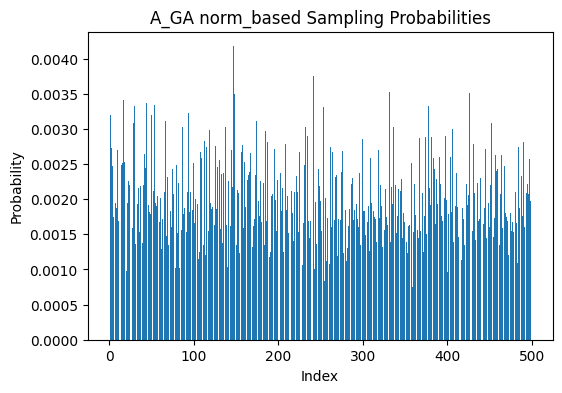
\includegraphics[width=0.5\textwidth]{/home/tagore/repos/STAT260/HW2/assets/Q9_A_GA norm_based Sampling Probabilities.png}
    \caption{GA Norm based probability distribution}
    \label{fig:GA_norm_based_prob}
\end{figure}

\begin{figure}[H]
    \centering
    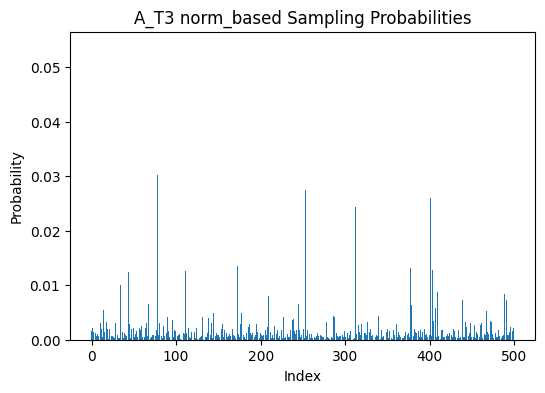
\includegraphics[width=0.5\textwidth]{/home/tagore/repos/STAT260/HW2/assets/Q9_A_T3 norm_based Sampling Probabilities.png}
    \caption{T3 Norm based probability distribution}
    \label{fig:T3_norm_based_prob}
\end{figure}

\begin{figure}[H]
    \centering
    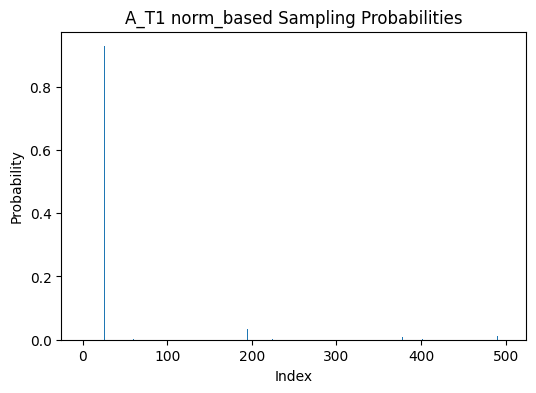
\includegraphics[width=0.5\textwidth]{/home/tagore/repos/STAT260/HW2/assets/Q9_A_T1 norm_based Sampling Probabilities.png}
    \caption{T1 Norm based probability distribution}
    \label{fig:T1_norm_based_prob}
\end{figure}

We will now plot the Frobenius and spectral error for the approximations of the three matrix multiplications.

\begin{figure}[H]
    \centering
    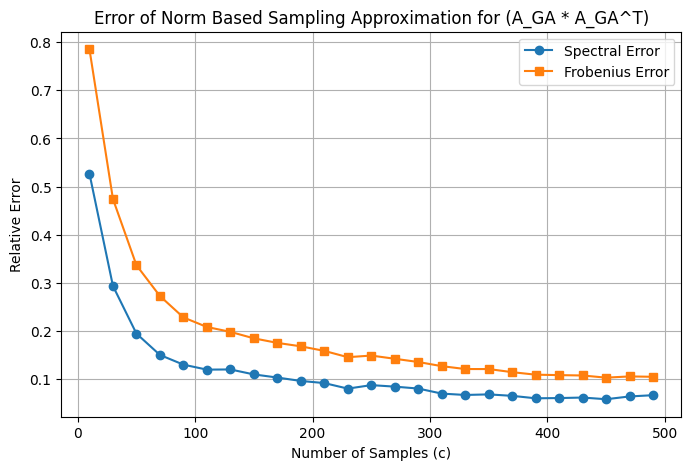
\includegraphics[width=0.5\textwidth]{/home/tagore/repos/STAT260/HW2/assets/Q9_Error of Norm Based Sampling Approximation for (A_GA * A_GA^T).png}
    \caption{Error of Norm Based Sampling Approximation for (\(A_{GA}^\top A_{GA}\))}
    \label{fig:GA_norm_based_error}
\end{figure}

\begin{figure}[H]
    \centering
    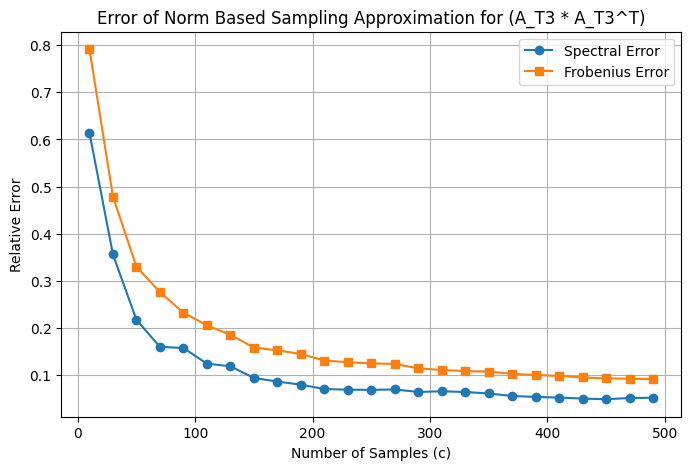
\includegraphics[width=0.5\textwidth]{/home/tagore/repos/STAT260/HW2/assets/Q9_Error of Norm Based Sampling Approximation for (A_T3 * A_T3^T).png}
    \caption{Error of Norm Based Sampling Approximation for (\(A_{T3}^\top A_{T3}\))}
    \label{fig:T3s_norm_based_error}
\end{figure}

\begin{figure}[H]
    \centering
    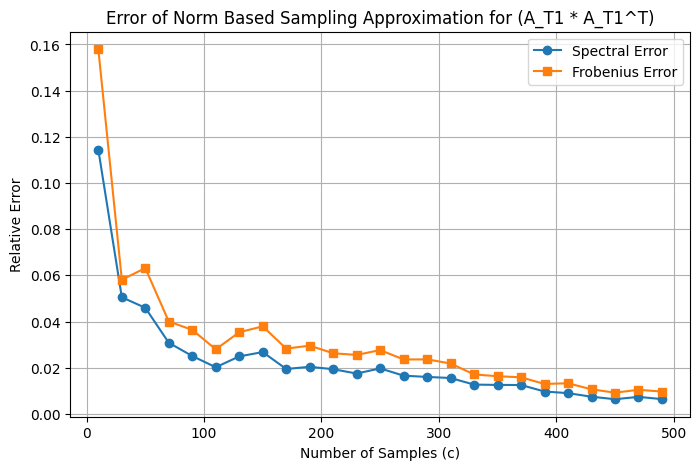
\includegraphics[width=0.5\textwidth]{/home/tagore/repos/STAT260/HW2/assets/Q_9_Error of Norm Based Sampling Approximation for (A_T1 * A_T1^T).png}
    \caption{Error of Norm Based Sampling Approximation for (\(A_{T1}^\top A_{T1}\))}
    \label{fig:T1_norm_based_error}
\end{figure}

\newpage

\section*{Problem 10}

We will now plot the Frobenius and spectral error for the approximations of the three left singular matrices multiplication.

\begin{figure}[H]
    \centering
    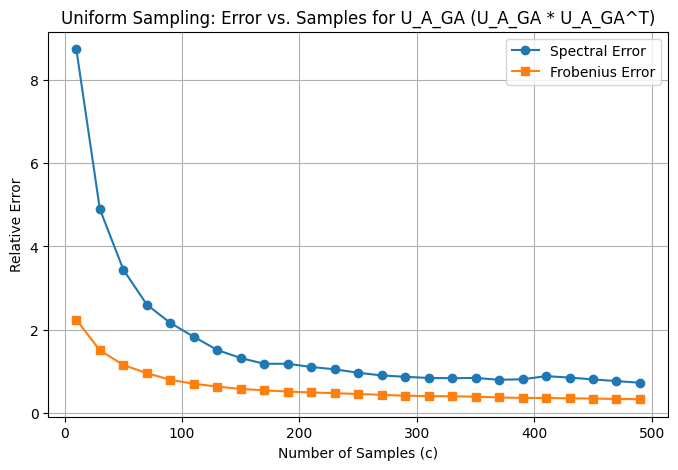
\includegraphics[width=0.5\textwidth]{/home/tagore/repos/STAT260/HW2/assets/Q10_Uniform Sampling: Error vs. Samples for U_A_GA (U_A_GA * U_A_GA^T).png}
    \caption{Error of Uniform Based Sampling Approximation for (\(U_{GA}^\top U_{GA}\))}
    \label{fig:GA_uniform_based_error}
\end{figure}

\begin{figure}[H]
    \centering
    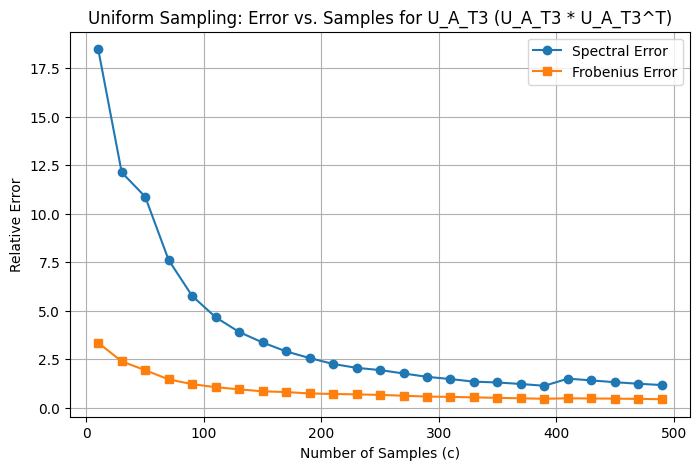
\includegraphics[width=0.5\textwidth]{/home/tagore/repos/STAT260/HW2/assets/Q10_Uniform Sampling: Error vs. Samples for U_A_T3 (U_A_T3 * U_A_T3^T).png}
    \caption{Error of Uniform Based Sampling Approximation for (\(U_{T3}^\top U_{T3}\))}
    \label{fig:T1_uniform_based_error}
\end{figure}

\begin{figure}[H]
    \centering
    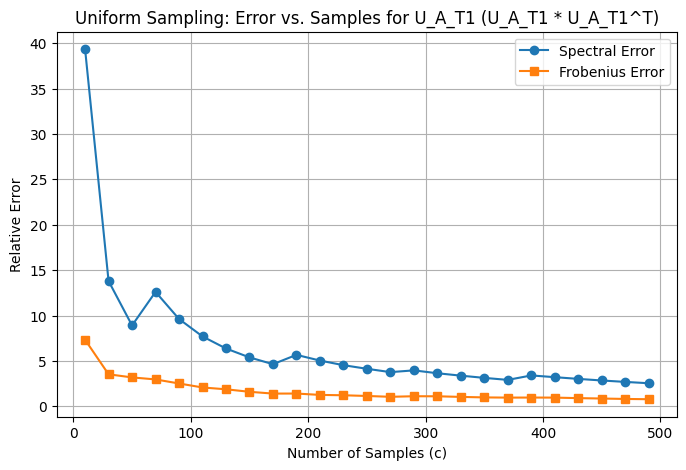
\includegraphics[width=0.5\textwidth]{/home/tagore/repos/STAT260/HW2/assets/Q10_Uniform Sampling: Error vs. Samples for U_A_T1 (U_A_T1 * U_A_T1^T).png}
    \caption{Error of Uniform Based Sampling Approximation for (\(U_{T1}^\top U_{T1}\))}
    \label{fig:T3_uniform_based_error}
\end{figure}

\newpage

\section*{Problem 11}

We will now plot the Frobenius and spectral error for the approximations of \(A^\top A\) using leverage score sampling.

\begin{figure}[H]
    \centering
    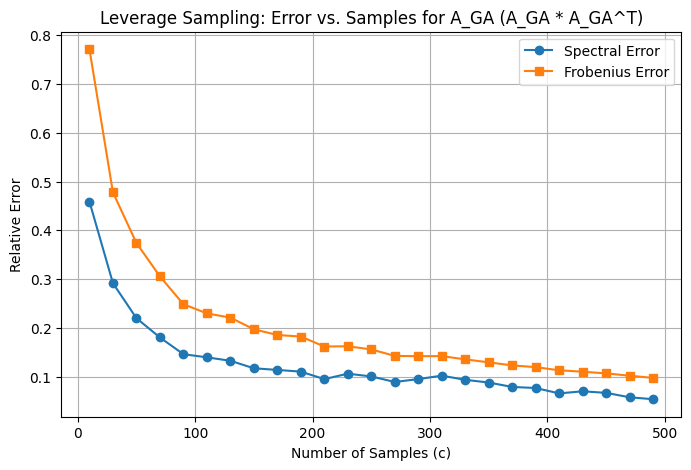
\includegraphics[width=0.5\textwidth]{/home/tagore/repos/STAT260/HW2/assets/Q11_Leverage Sampling: Error vs. Samples for A_GA (A_GA * A_GA^T).png}
    \caption{Error of Leverage Based Sampling Approximation for (\(A_{GA}^\top A_{GA}\))}
    \label{fig:GA_leverage_based_error}
\end{figure}

\begin{figure}[H]
    \centering
    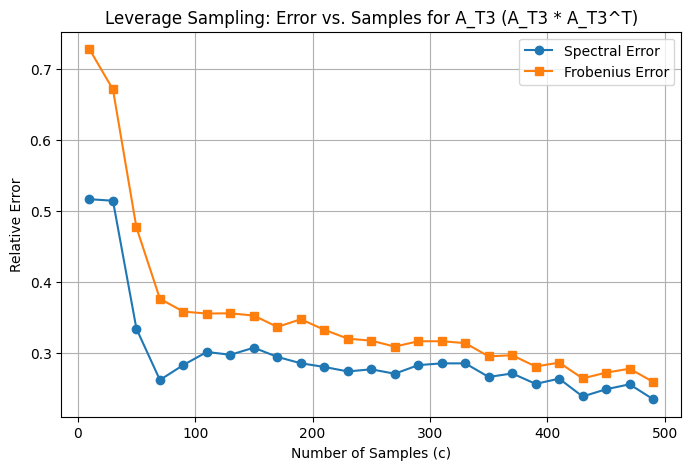
\includegraphics[width=0.5\textwidth]{/home/tagore/repos/STAT260/HW2/assets/Q11_Leverage Sampling: Error vs. Samples for A_T3 (A_T3 * A_T3^T).png}
    \caption{Error of Leverage Based Sampling Approximation for (\(A_{T3}^\top A_{T3}\))}
    \label{fig:T1_leverage_based_error}
\end{figure}

\begin{figure}[H]
    \centering
    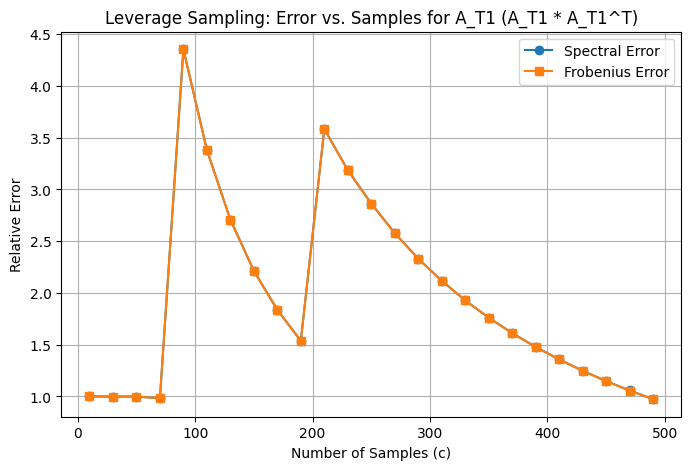
\includegraphics[width=0.5\textwidth]{/home/tagore/repos/STAT260/HW2/assets/Q11_Leverage Sampling: Error vs. Samples for A_T1 (A_T1 * A_T1^T).png}
    \caption{Error of Leverage Based Sampling Approximation for (\(A_{T1}^\top A_{T1}\))}
    \label{fig:T3_leverage_based_error}
\end{figure}

The results looks similar for $A_{GA}$ and $A_{T3}$, but the error for $A_{T1}$ is significantly higher than the other two matrices. 
This means that the leverage score sampling is not as effective for $A_{T1}$ as it is for the other two matrices.


\section*{Problem 12}



% \section*{Problem 2}
% Here is an example of a graph:
% \begin{figure}[h!]
%     \centering
%     \includegraphics[width=0.5\textwidth]{example-graph.png}
%     \caption{Example Graph}
%     \label{fig:example-graph}
% \end{figure}

\end{document}